\section{Motivation}
\subsection{Milit�rische Lage}
\begin{frame}\frametitle{Lagebeispiel}  

 \begin{columns}[t]
\begin{column}{5cm}
  \begin{block}{2 eigene Panzer (blau)}
    \begin{itemize}[<+-| alert@+>]
  	  \item bewegen sich nicht
  	  \item melden Beobachtungen in konstanten Zeitabst�nden
    \end{itemize}
  \end{block}\end{column}
\begin{column}{5cm}
  \begin{block}{2 feindliche Panzer (rot)}
  \begin{itemize}[<+-| alert@+>]
  	\item ein Panzer in Querfahrt
  	\item ein Panzer in in Richtung der eigenen Kr�fte
    \end{itemize}
\end{block}\end{column}
\end{columns}
\end{frame}

\begin{frame}\frametitle{Darstellung der Beispiellage}
\begin{figure}[h]
	\centering
		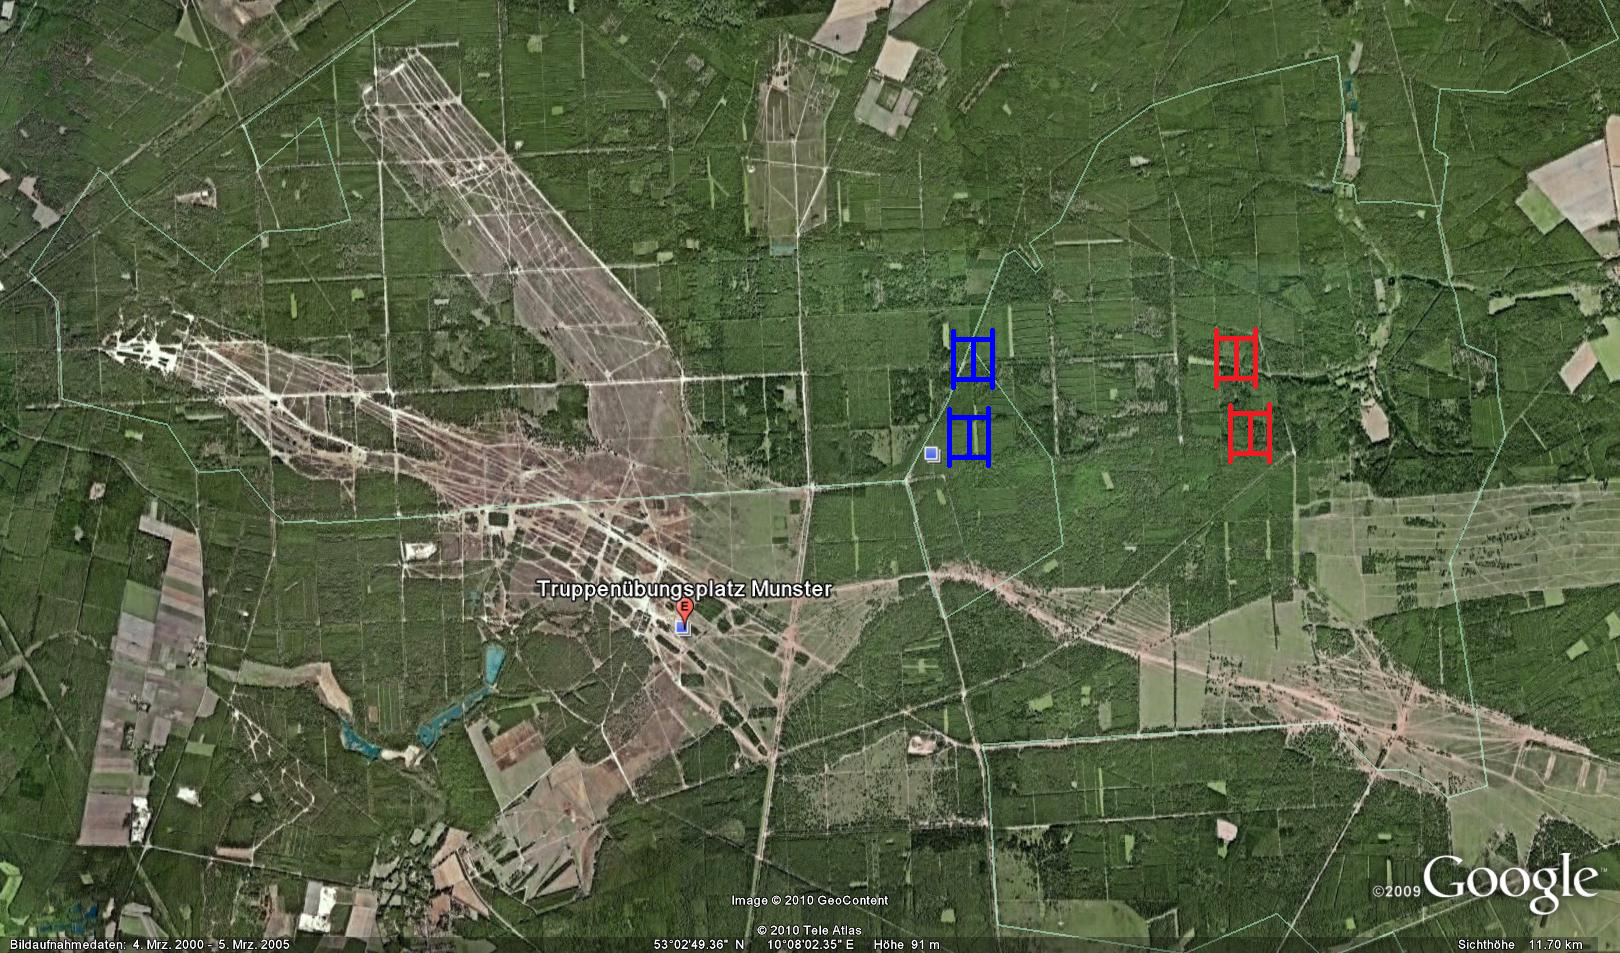
\includegraphics[width=0.80\textwidth]{Bilder/googleearth.png}
	\caption{Lage zum ersten Meldezeitpunkt}
	\label{fig:googleearth}
\end{figure}
\end{frame}

\begin{frame}\frametitle{Darstellung der Beispiellage}
\begin{figure}[h]
	\centering
		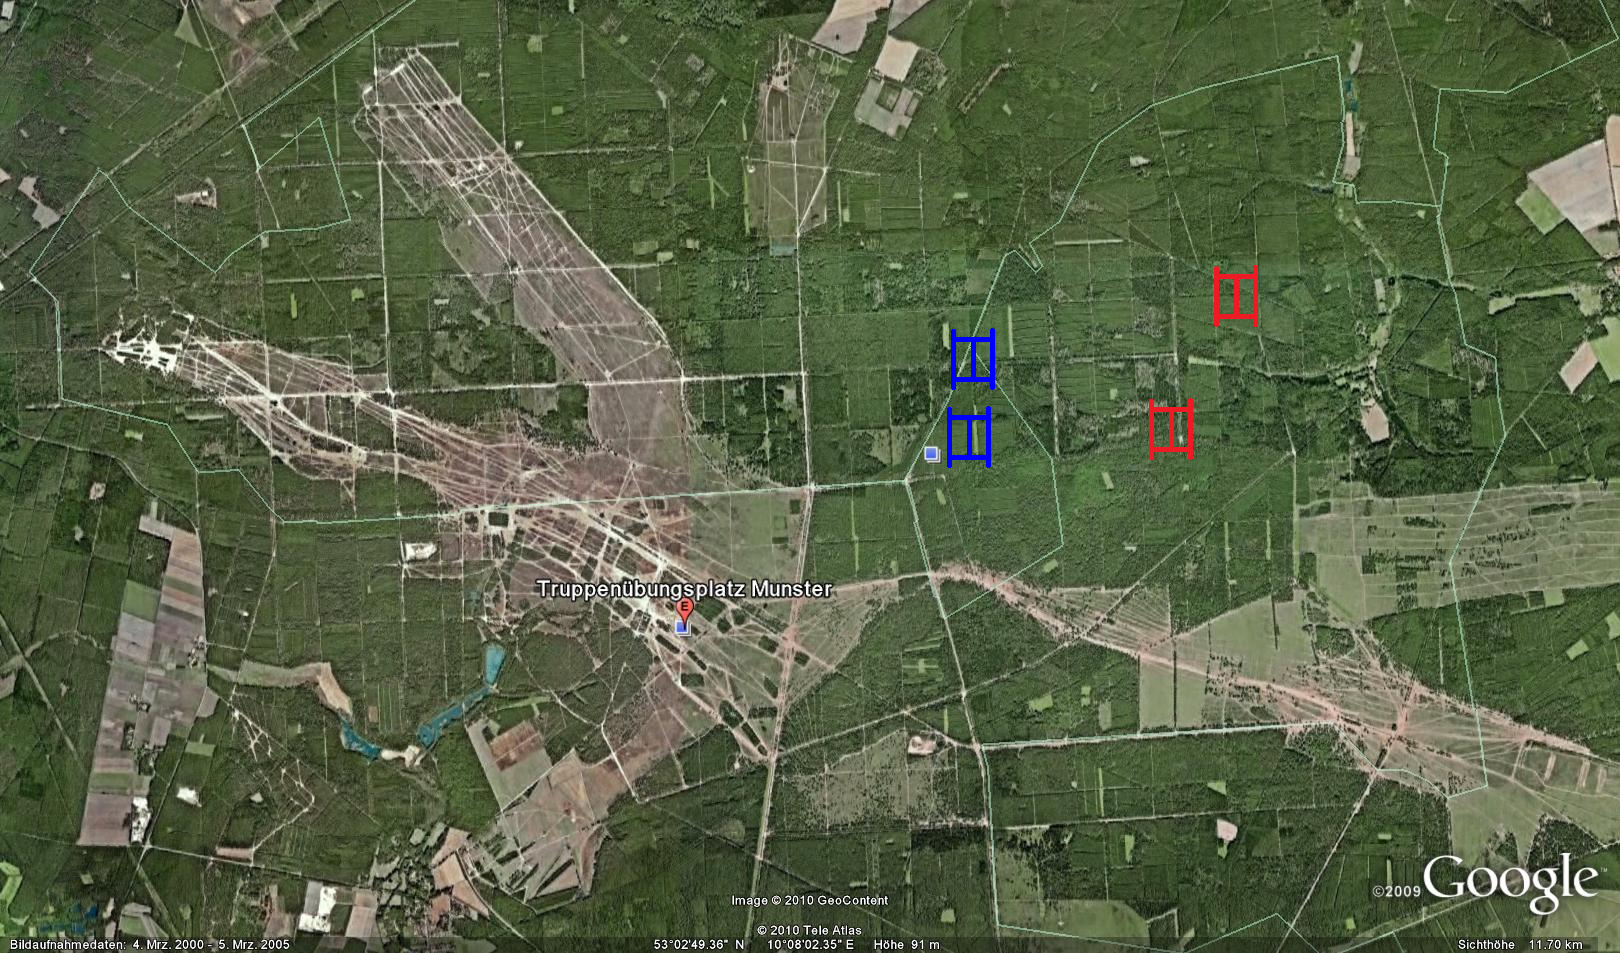
\includegraphics[width=0.80\textwidth]{Bilder/googleearth2.png}
	\caption{Lage zum zweiten Meldezeitpunkt}
	\label{fig:googleearth2}
\end{figure}
\end{frame}

\begin{frame}\frametitle{Darstellung der Beispiellage}
\begin{figure}[h]
	\centering
		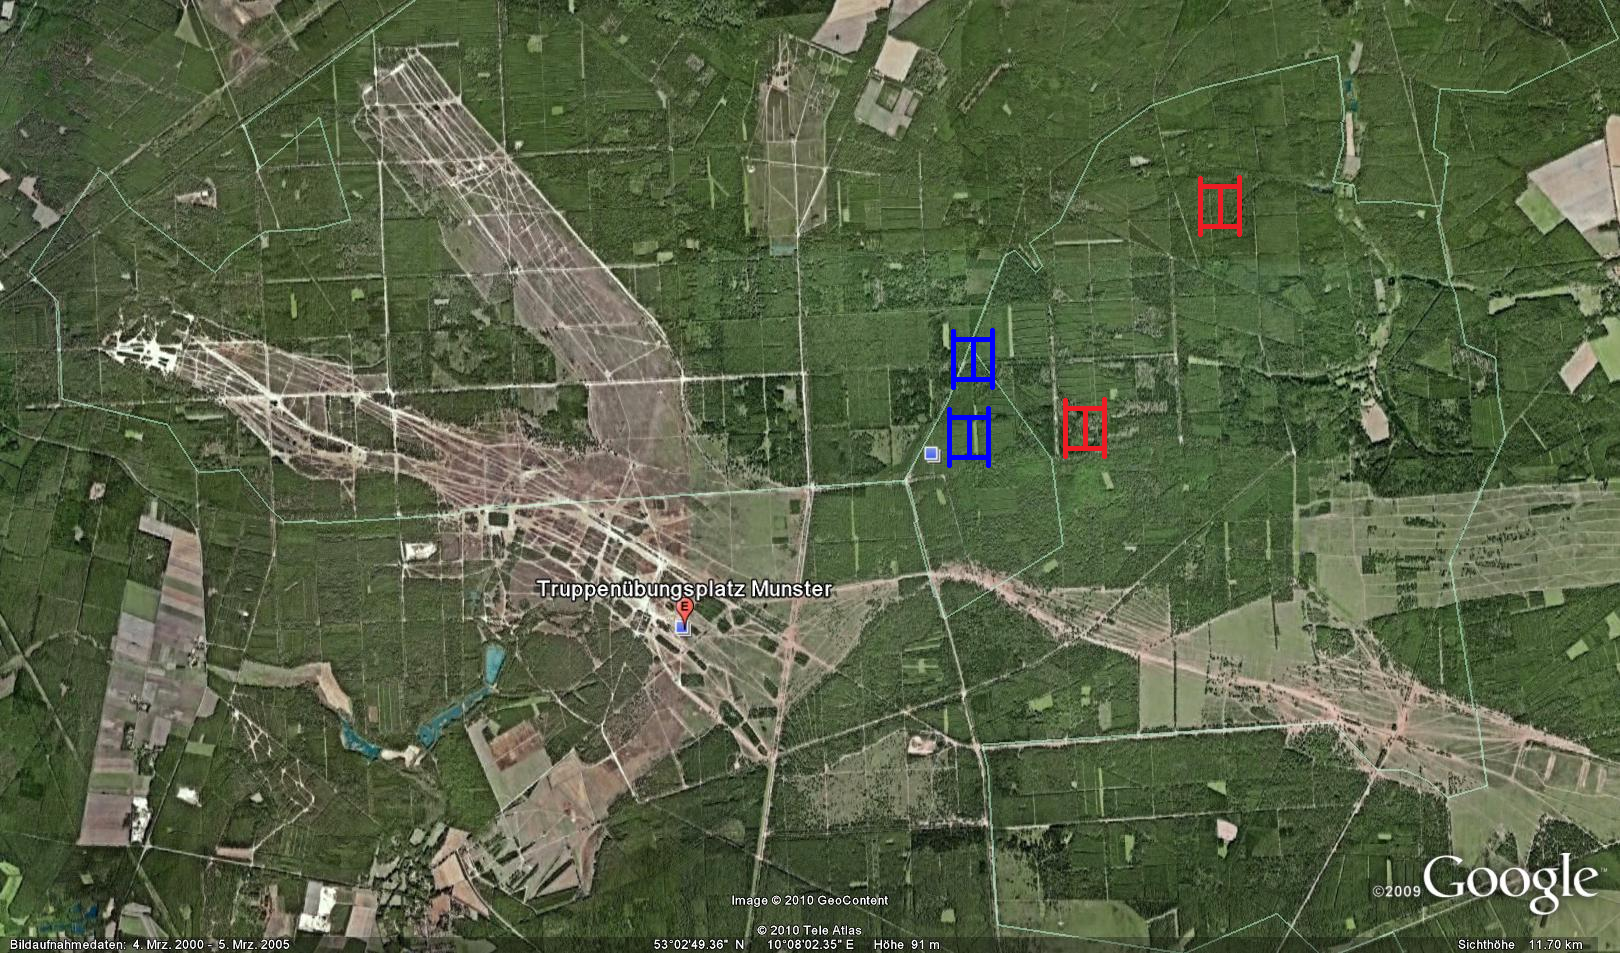
\includegraphics[width=0.80\textwidth]{Bilder/googleearth3.png}
	\caption{Lage zum dritten Meldezeitpunkt}
	\label{fig:googleearth3}
\end{figure}
\end{frame}

\subsection{Repr�sentation der Daten}

\begin{frame}[fragile]
\frametitle{Darstellung der Meldungen in XML}
\lstset{%
language=XML,
basicstyle={\ttfamily \tiny},
numbers=left,                   % where to put the line-numbers
numberstyle=\tiny,      % the size of the fonts that are used for the line-numbers
stepnumber=1
}%
\begin{lstlisting}[breaklines=true,frame=tlRB,captionpos=b,caption={Darstellung einer Meldung in XML}] 
<Situation>
  <Units>
   <Unit>
      <Name>FriendlyTank1</Name>
      <Location>
        <Lat>52.796629714678467</Lat>
        <Lon>9.89990561649954</Lon>
        <LastModified>2009-02-20T10:25:36+01:00</LastModified>
      </Location>
    </Unit>
    <Unit>
      <Name>FriendlyTank2</Name>
      <Location>
        <Lat>52.794038961891268</Lat>
        <Lon>9.9011727699025922</Lon>
        <LastModified>2009-02-20T10:25:36+01:00</LastModified>
      </Location>
    </Unit>
  </Units>
</Situation>
\end{lstlisting}
\end{frame}

\subsection{Problemstellung}

\begin{frame}\frametitle{Problemstellung}

\begin{block}{Redundante Meldungen zu einem Objekt}
\begin{itemize}[<+-| alert@+>]
    \item Sichtung unterschiedlicher Beobachter zur selben Zeit
    \item Sichtung zu unterschiedlichen Zeiten
\end{itemize}
\end{block}
\begin{itemize}[<+-| alert@+>]
    \item Redundanzen verf�lschen die Lage
    \item Weiterverarbeitung und Analyse unm�glich
    \item \textbf{Beseitigung der Redundanzen ist notwendig}
\end{itemize}
\end{frame}

